
\chapter{Biophysical validation}

\section{The challenge with sequencing}

The ability to generate large amounts of RNA-protein interaction data using CLIP-seq is useful \cite{Konig:2012ww}. But, how can be distinguish between bona-fide signal and artifacts products by non-specific molecular interactions? To date, our applications of CLIP relied on three approaches: (1) enforcing experimental replicates and merging reads from each \cite{Flynn:2014bi}, (2) standardized output data types that ease comparative analysis between datasets and make it easy to exclude genes with redundant, nonspecific binding patters \cite{Flynn:2014bi}, and (3) experimental validation of hypotheses  \cite{Calo:2014ix}. 

\section{Highly multiplexed validation}

We developed an additional method of validation, which takes advantage of microfluidic tools that enable highly multiplexed measurements of interaction affinity. Specifically, we adapted the MITOMI \cite{Fordyce:2010fb} microfluidic platform such that an entire RNA library (e.g., every RNA identified via CLIP) could be simultaneously synthesized and assayed for ligand-binding \cite{Martin:2012cx}. This technique, termed RNA-MITOMI, is thus complementary with sequencing-based methods for RNA interactomics (such as CLIP) because thousands of putative RNA-ligand interactions can be evaluated.

\begin{figure*}
\center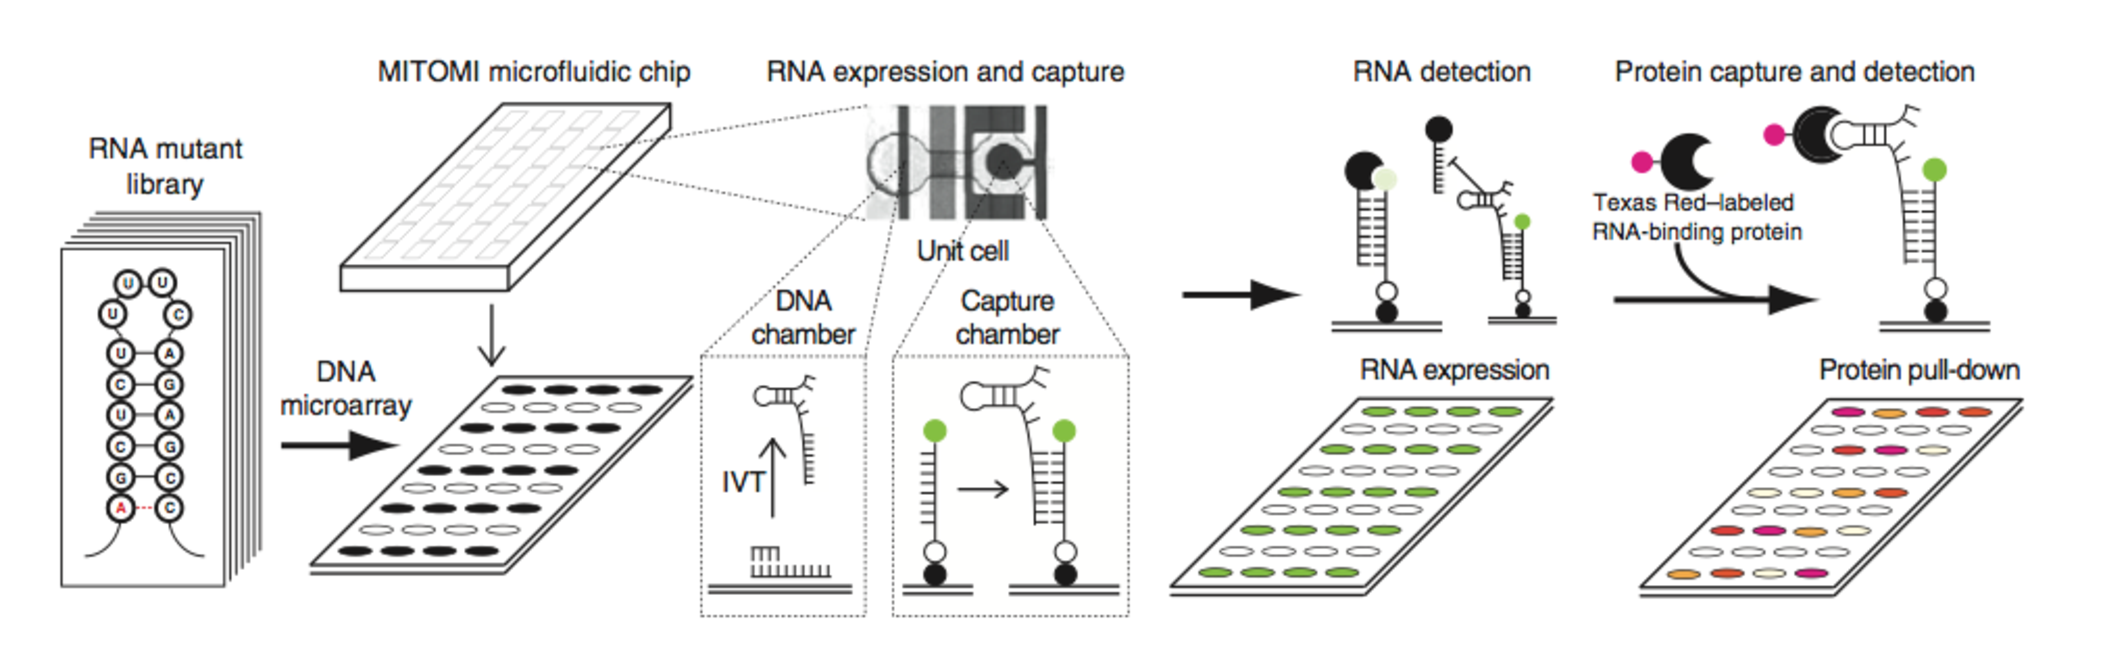
\includegraphics[width=150mm,scale=0.5]{Figures/Fig28}
\caption{MITOMI assay design.}
\label{fig:Fig28}
\end{figure*}

The MITOMI microfluidic chip used in this study has 640 microchambers, each with a volume $\approx$1 nl. We arrayed DNA oligos, which serve as transcription templates for the RNA library, and overlaid the MITOMI chip onto the array such that each spot was compartmentalized in a unique microchamber. Each chamber has a back-chamber, which houses the spotted DNA template, and a detection chamber in which the interaction between RNA and ligand is measured (Figure ~\ref{fig:Fig28}).

\section{Stem loop binding protein}

We applied this strategy to the well-characterized interaction between stem-loop binding protein (SLBP) and the 3$'$ histone mRNA stem-loop \cite{Marzluff:2008fy}. We measured relative SLBP binding across our library of single and double RNA mutants at 3 nM protein concentration (Figure ~\ref{fig:Fig29}). With this data, we identified three functional three regimes: 15 mutants had little effect on binding, 15 deleterious mutants were rescued by compensatory mutations that restore RNA structure, but three mutants could not be rescued by restoring structure, indicating sequence-based recognition at these positions. We used the data set to to distill sequence and structural requirements for stem-loop function (SLBP binding) at single-nucleotide resolution.

\begin{figure*}
\center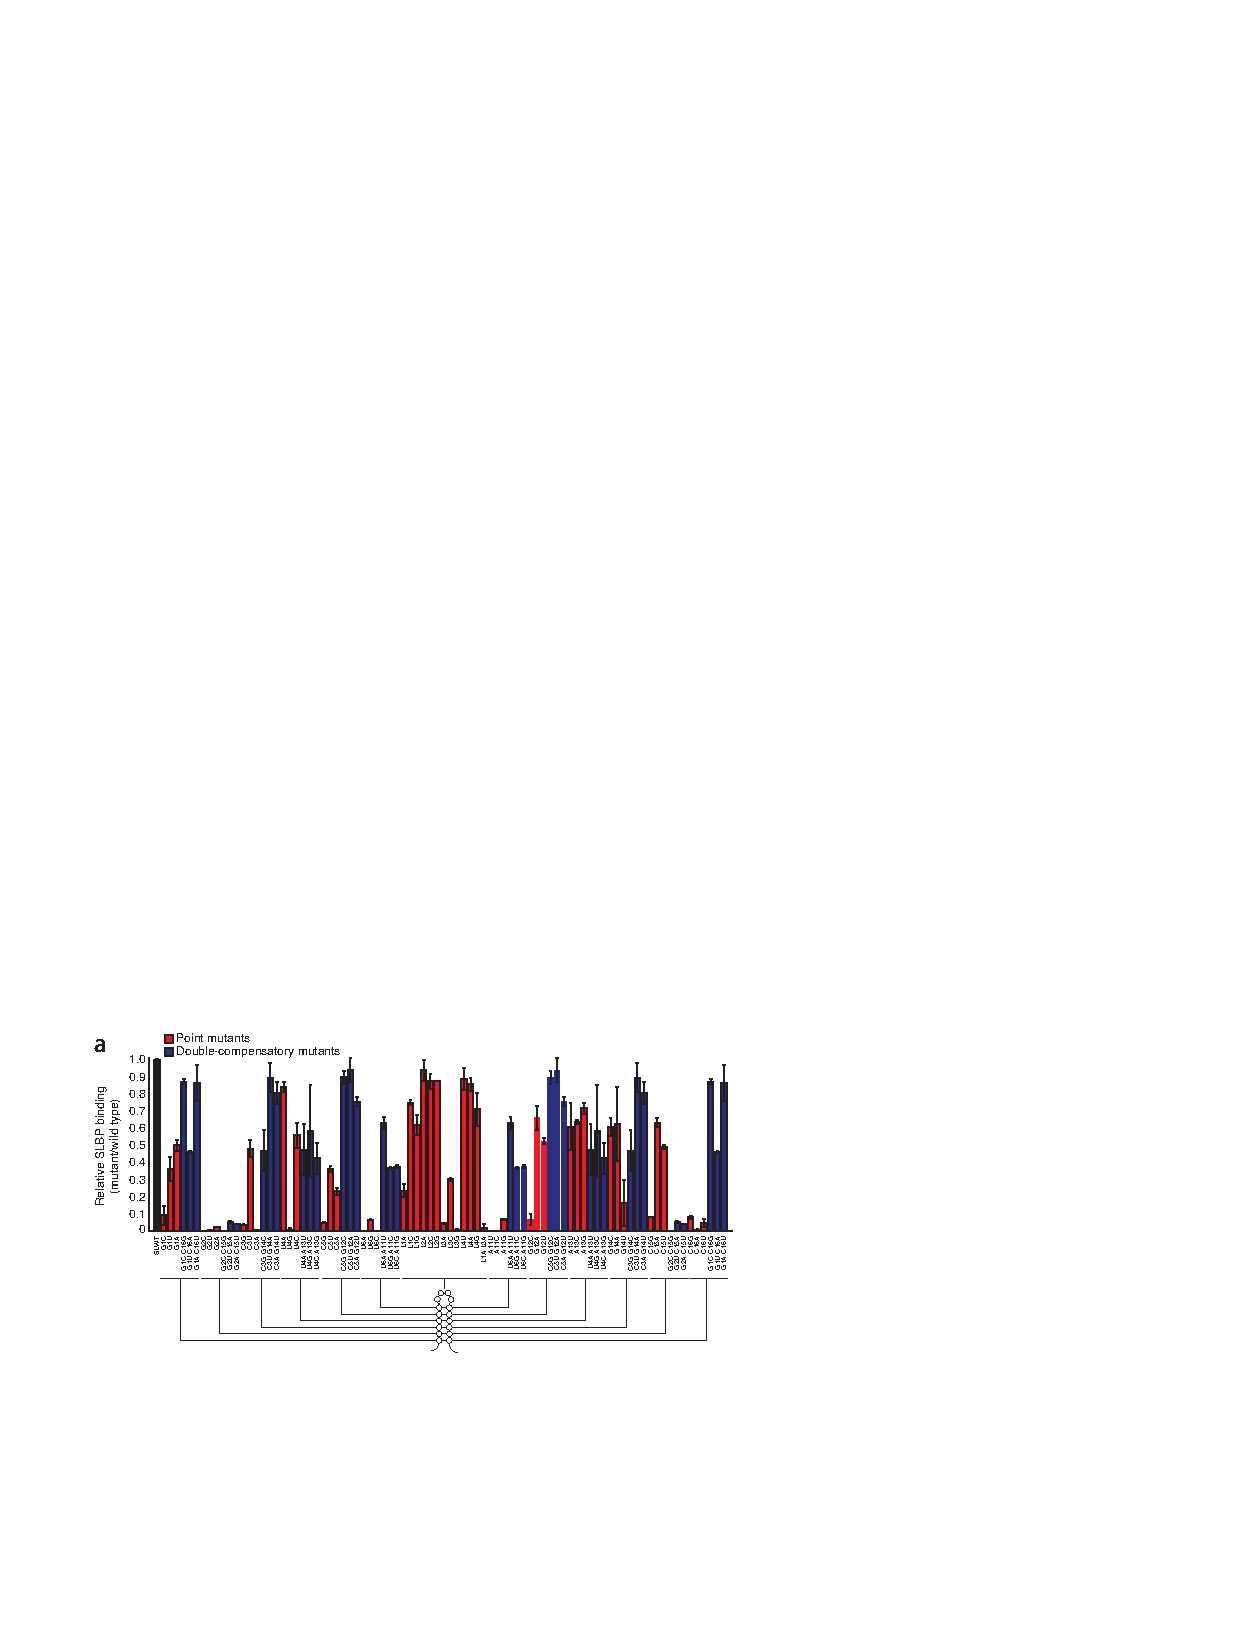
\includegraphics[width=150mm,scale=0.5]{Figures/Fig29}
\caption{Multiplexed measurement of affinity.}
\label{fig:Fig29}
\end{figure*} 
 
 We validated the data in two ways. First, the features identified in the functional motif recapitulated the pattern of phylogenetic conservation of stem-loop sequences, suggesting that SLBP binding is the dominant selective constraint on the histone 3$'$ end. Residues (G2 and U9) and structural features (the U6 - A11 base pair) that are critical for SLBP binding are conserved from Tetrahymena sp. to humans, whereas we observed covariation for base pairs that have less stringent sequence-specificity \cite{Marzluff:2008fy}. Second, we tested nine point mutants with electrophoretic mobility shift analysis. The shift data agreed with the measurement of binding affinity obtained with RNA-MITOMI, confirming that measurements on the MITOMI platform can be recapitulated with conventional biochemical assays.
 
 \begin{figure*}
\center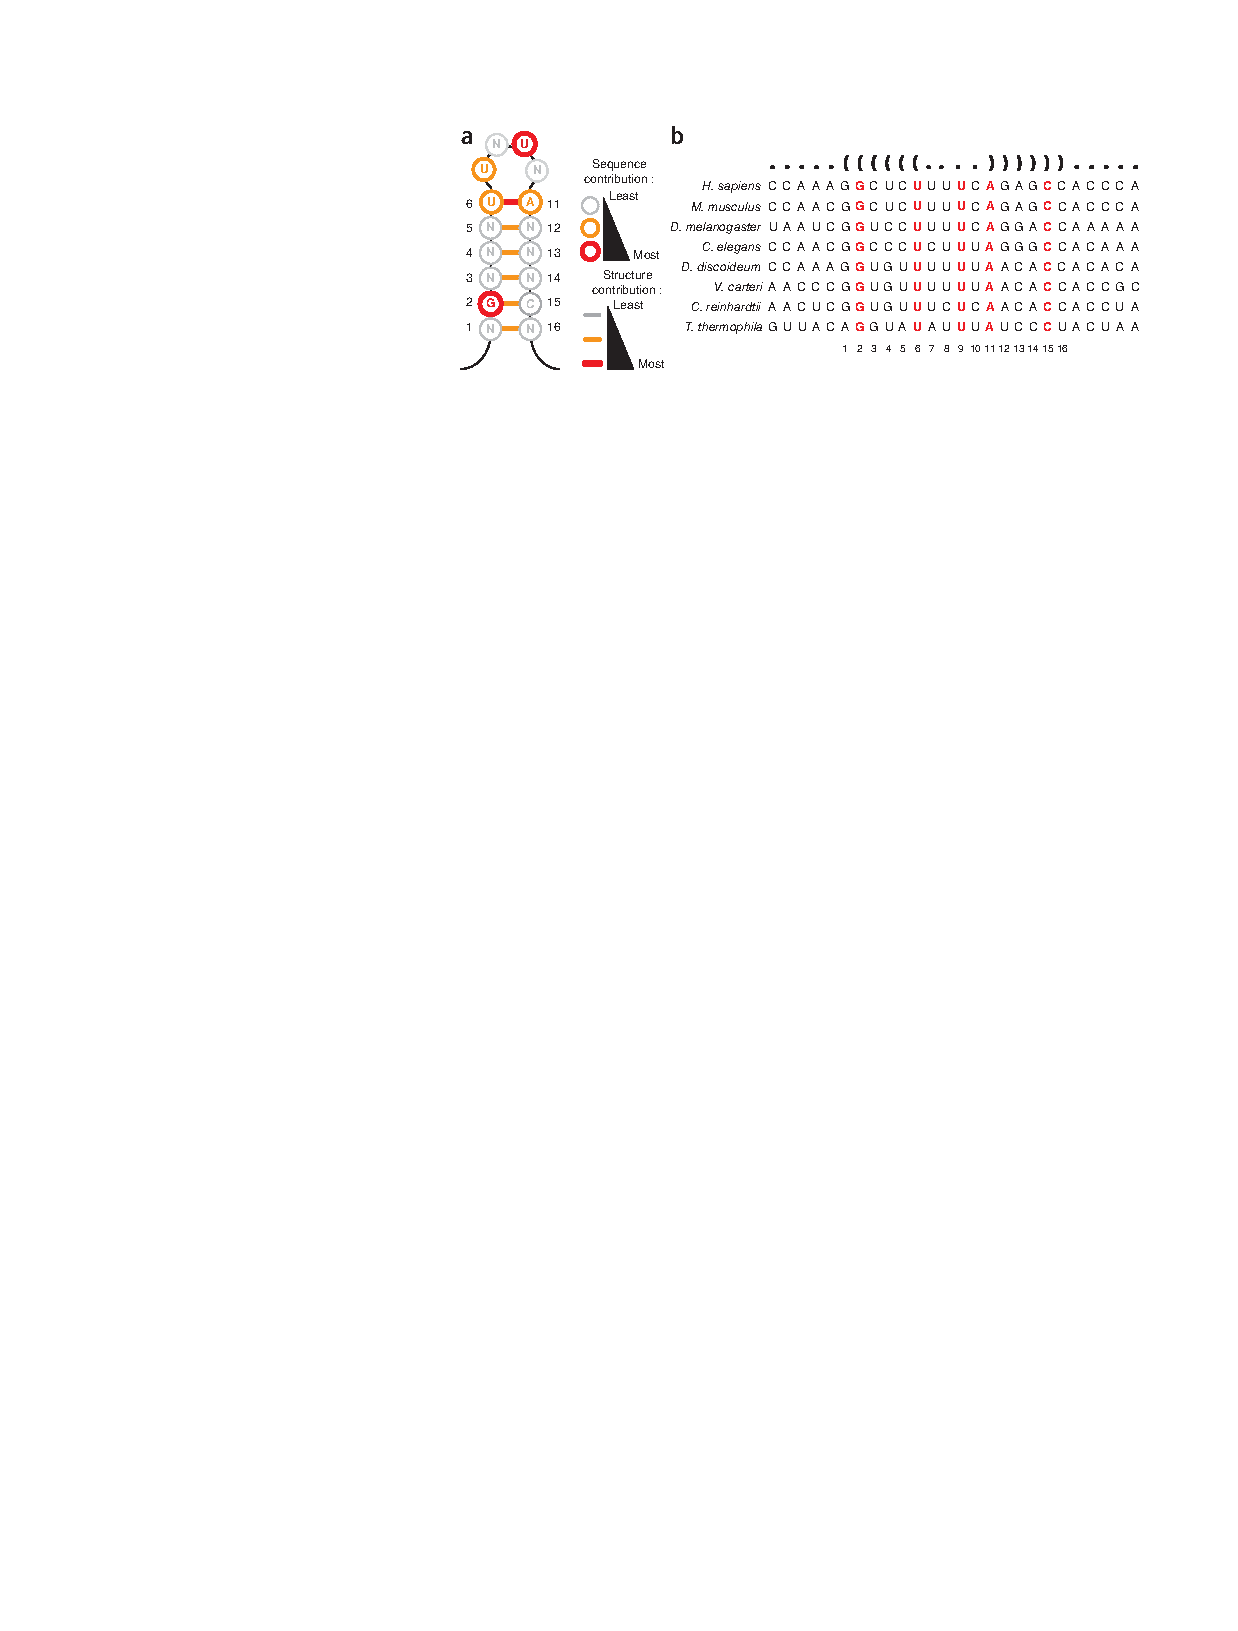
\includegraphics[width=150mm,scale=0.5]{Figures/Fig30}
\caption{Function RNA motifs.}
\label{fig:Fig30}
\end{figure*} 
 
Our results show that SLBP recognizes much of the stem via RNA secondary structure rather than sequence (Figure ~\ref{fig:Fig30}). For nine of the 12 bases in the stem, function was not dependent on sequence, as individual base-pair substitutions at these positions were tolerated. In some cases, base substitutions were functionally neutral only if structure was preserved. In particular, Watson-Crick base pairing is required at the U6-A11 position at the top of the stem. Nucleotide-specific contacts are also important for SLBP binding. Consistent with prior studies, two residues in the loop (U7 and especially U9) as well as G2 in the stem are required for binding.

Extending the results from prior studies, using our panel of mutants we also identified noncanonical base pairs that are tolerated. Though the G2?C15 base pair cannot be replaced by any of the three Watson-Crick base pairs, base substitutions in the position (C15) opposing G2 are tolerated, as mutations that allow wobble base-pairing (C15U) or prevent Watson-Crick base pairing (C15A) had nearly wild-type binding. Similar to the C15A mutation, C5A established a functionally tolerated G-A base pair. In addition, G12A and G1A mutations created a functionally tolerated A-C pair and G14C created a tolerated C-C. These noncanonical pairs can be deleterious if combined, suggesting limited tolerance to structure perturbation in the stem. 

\section{Summary}

Highly multiplexed biophysical methods, such as MITOMI, can overcome the gap between high sequencing throughput and the conventionally low throughput of biophysical assays, such as gel-shift. Recently, these assays have be re-purposed on sequencing flow-cell \cite{Buenrostro:2014kx}, which suggests that read-out of CLIP-seq data could be followed directly by validation of biophysics on the same sequencing platform.


 
 
 